\chapter{1D Positional Experiments - 2 Categories}

\section{Experimental Setup}

\section{2 Category Decisions}

\section{Dataset}

\section{Initial Analysis}

\ref{Figure:bar_responses_LR} shows a bar chart of the responses at each position. 
At position $0.5$, the number and of left and right responses were found to be exactly equal.
 At points away from the centre, the number of left or right responses at each position remains near constant.
  This indicates that there is a sharp transition from left to right ( for most workers) as the position of the circle is increased from $0 - 1$. 
  There is little ambiguity or fuzziness in the workers' responses. 


\begin{figure}
	\centering
	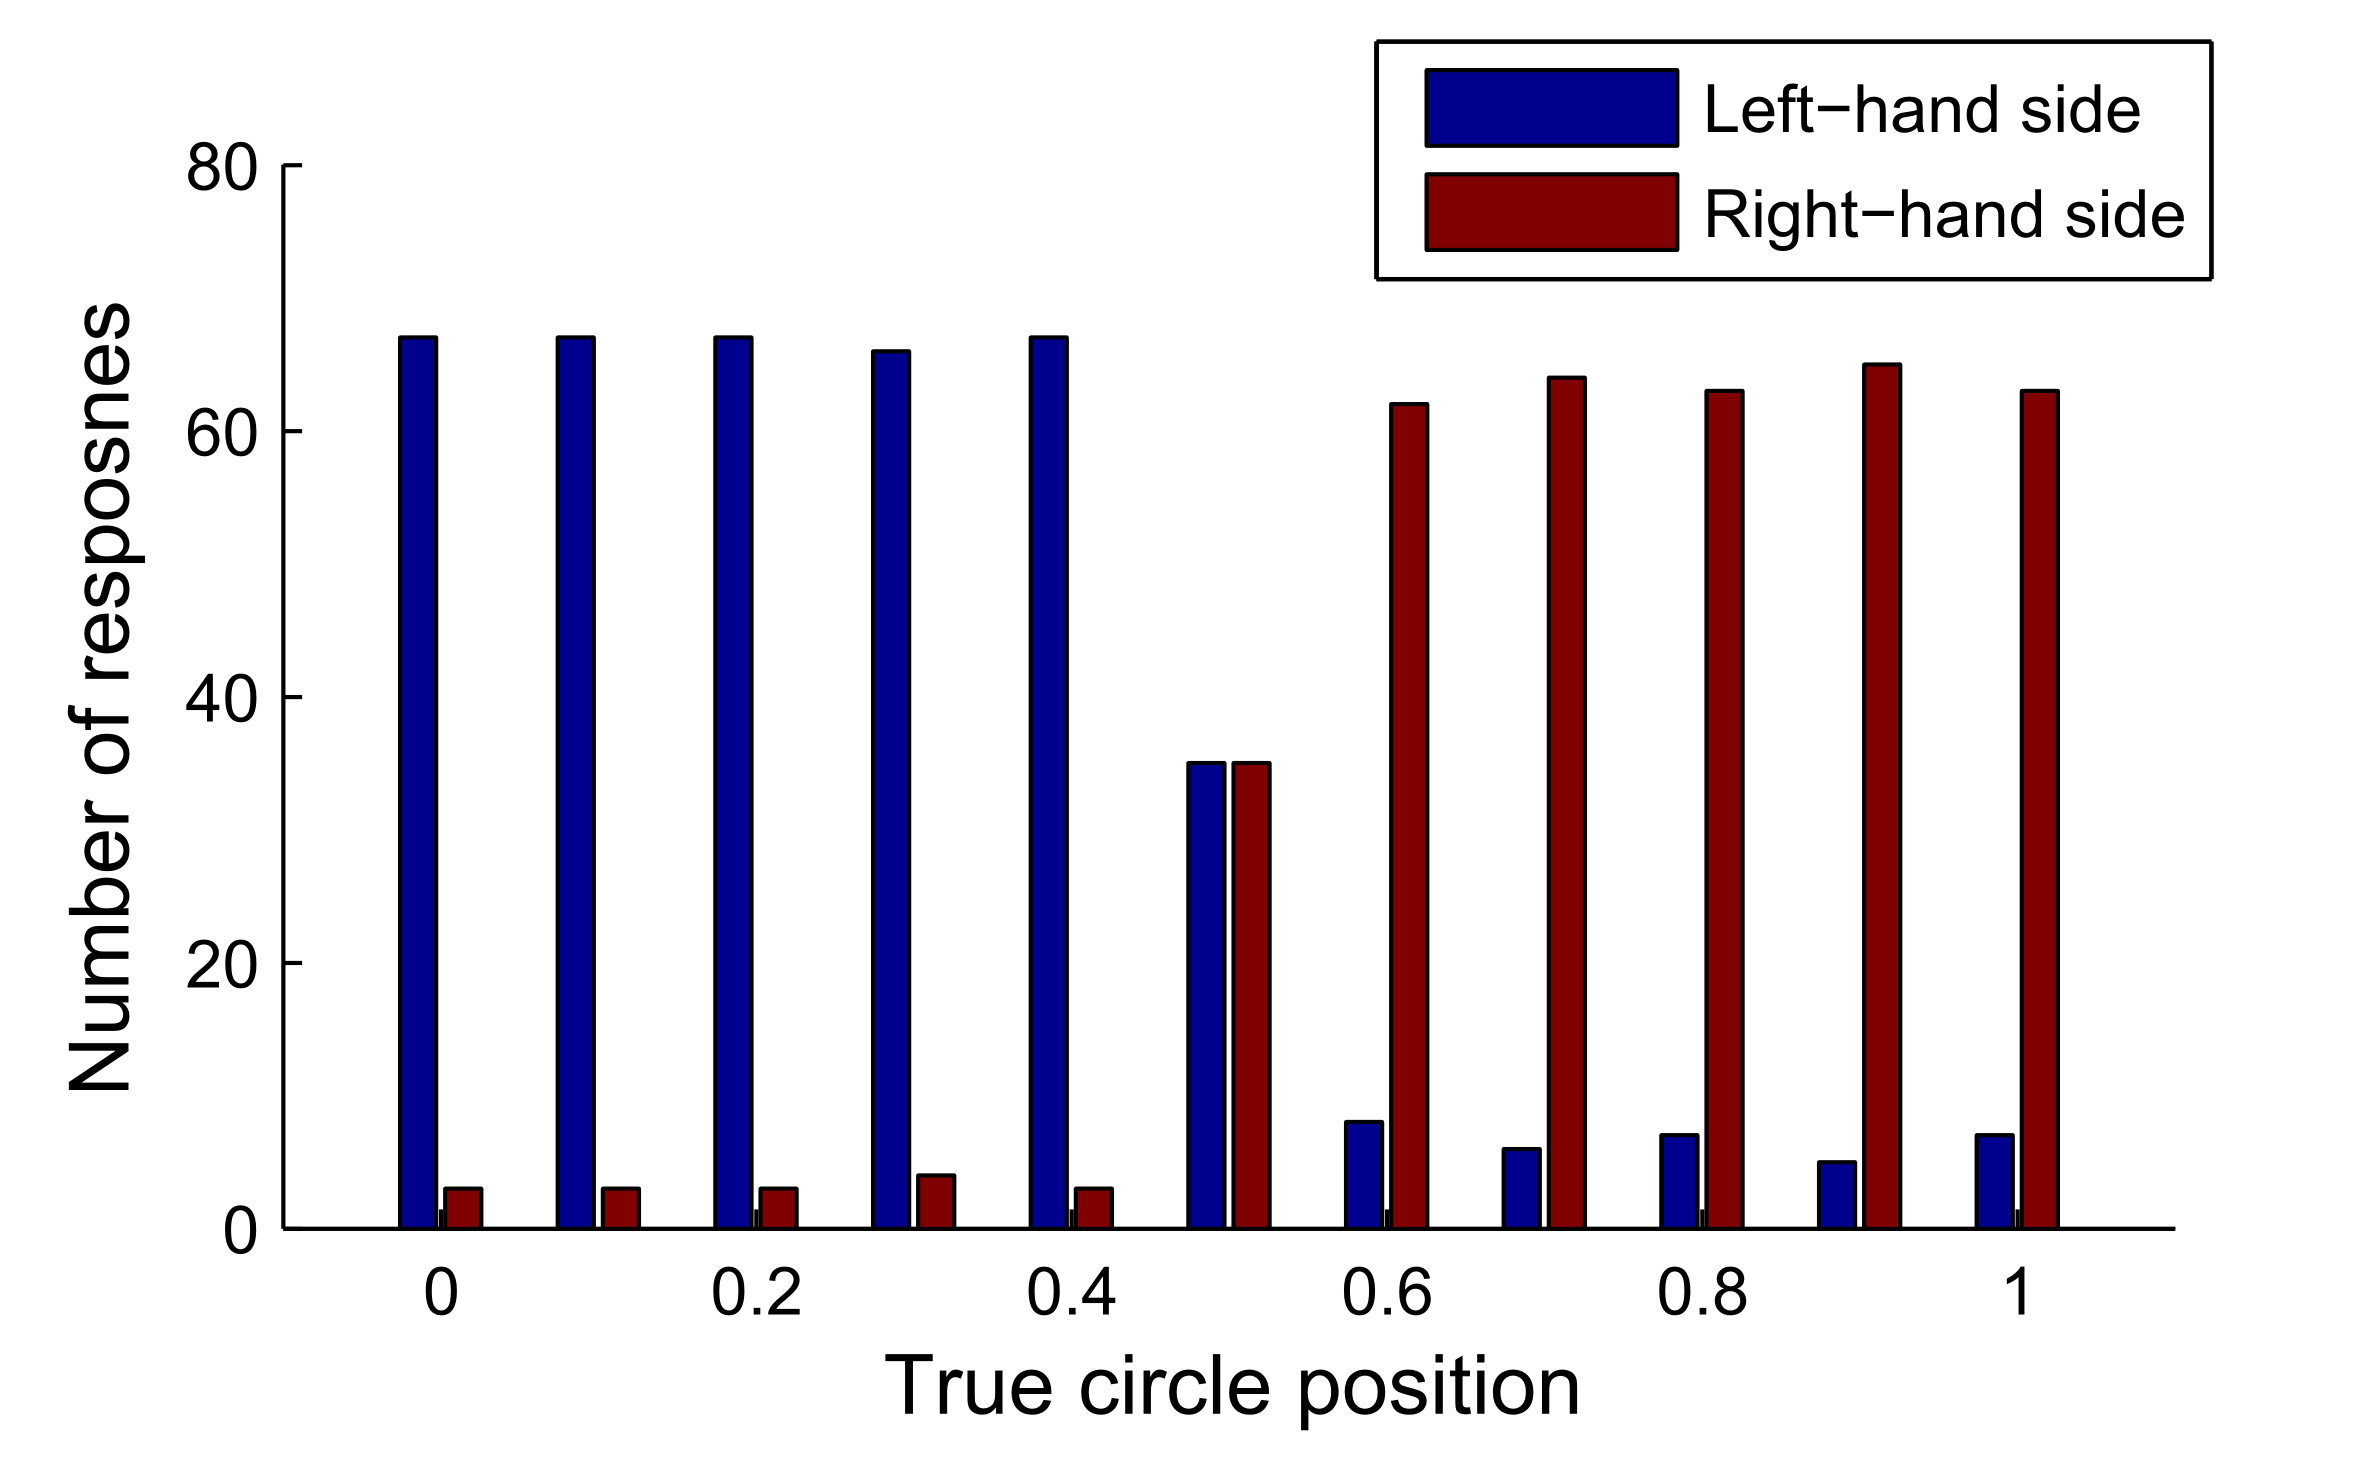
\includegraphics[scale=1]{bar_responsesLR.png}
	\caption{The number of left and right responses at each circle position. The total number of workers is 70.}
	\label{Figure:bar_responses_LR}
\end{figure}


\subsection{Non-gold responses}

We can apply simple gold standard data filtering to the dataset. 
By setting the extreme values of the circle position at 0 and 1 to gold standard data, we can filter out some workers. 
A total of 7 workers, or 10\% of the dataset, were filtered out. 
\ref{Figure: not_gold_responsesLR} shows the workers that were filtered out. 
In \ref{Figure: line_not_gold_responseLR} we can see the response models of the individual workers. 
Some show the opposite from what we might expect, by responding `Left-hand side' when the circle was on the far right. 
This suggests that they have not understood the answer they are giving. 
\ref{Figure: bar_not_goldLR} shows the responses at each circle position for 


\begin{figure}
	\centering
	\begin{subfigure}{7cm}
	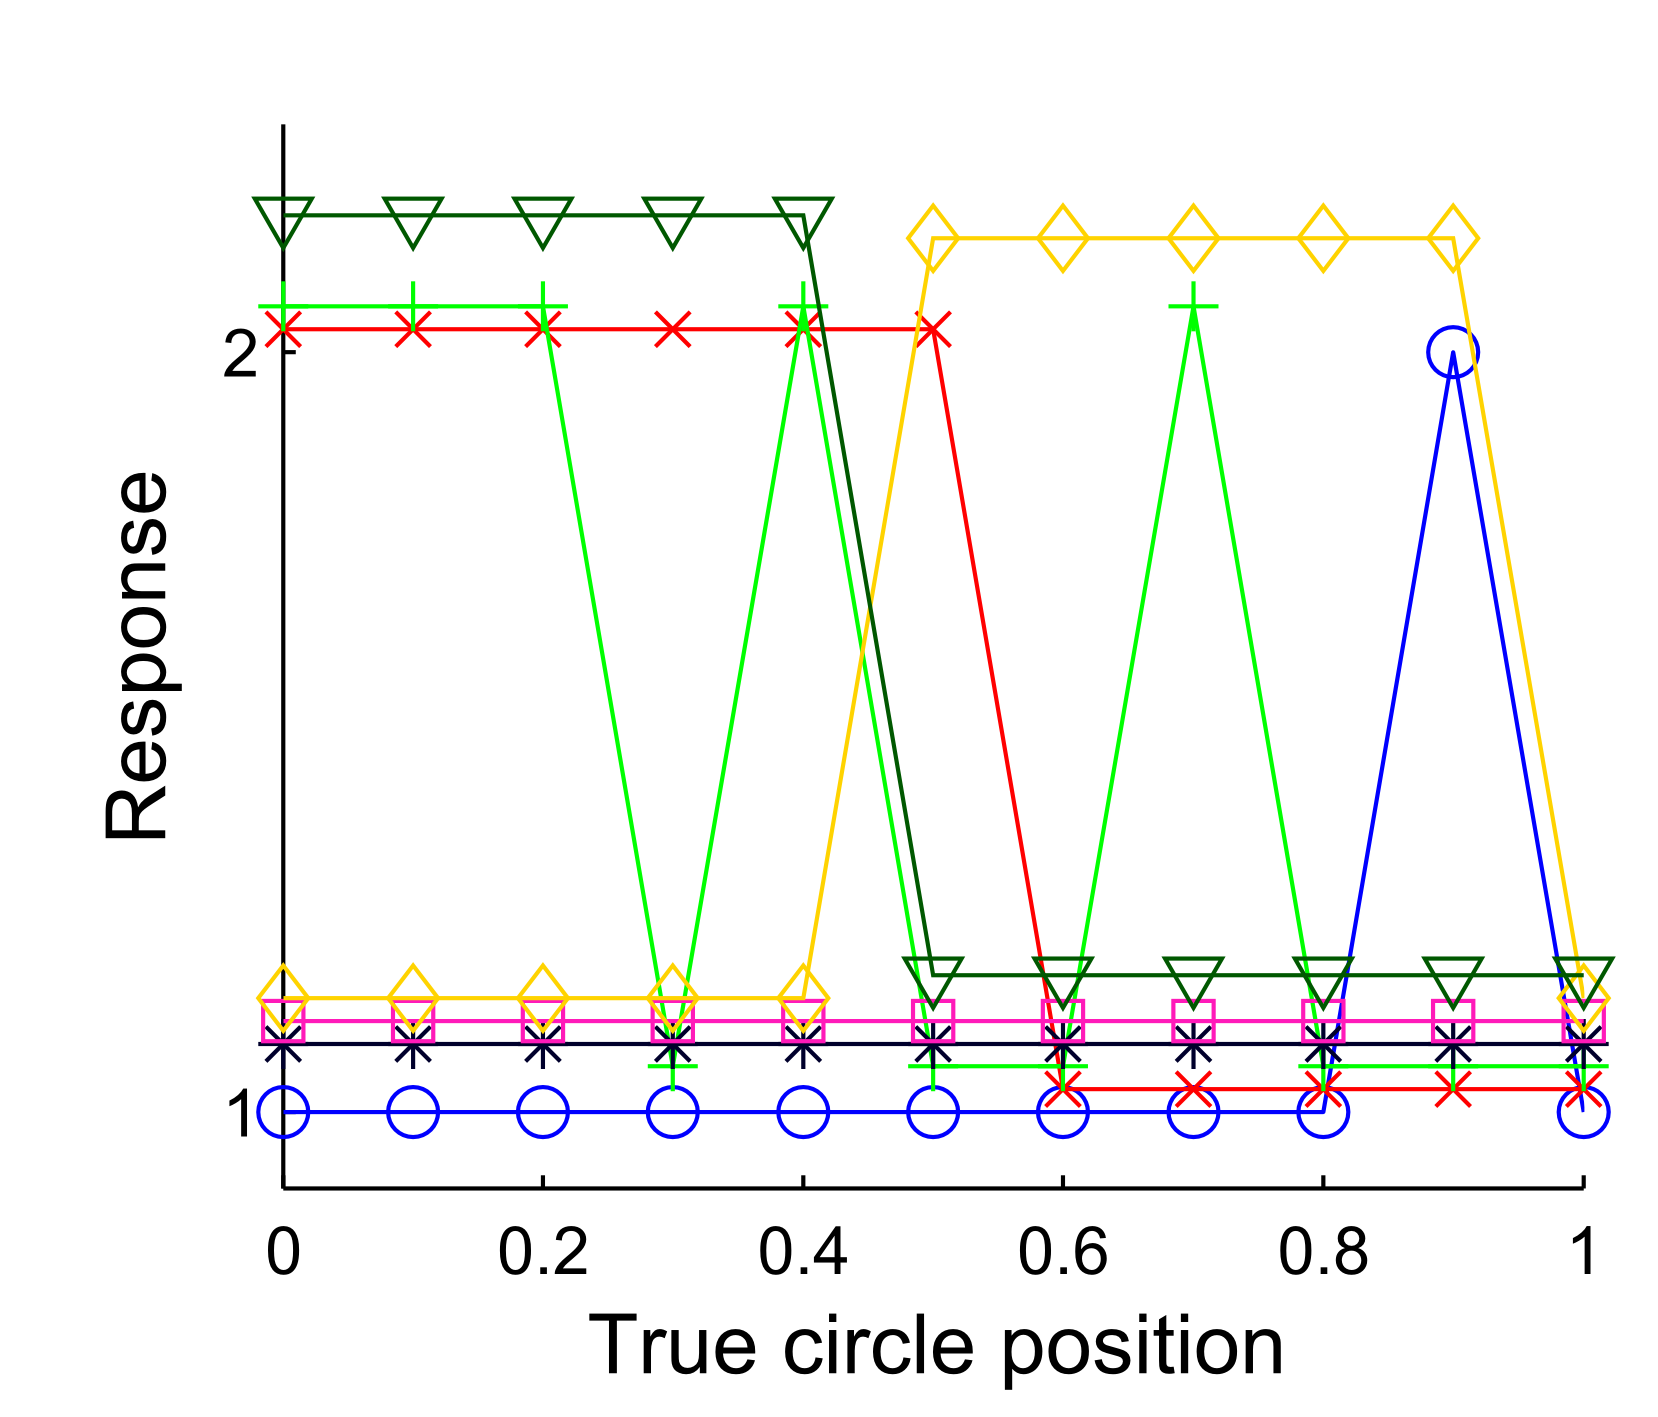
\includegraphics[scale=1]{line_not_gold_response_curves.png}
	\caption{}	
	\label{Figure: line_not_gold_responseLR}
	\end{subfigure}
	\begin{subfigure}{7cm}
	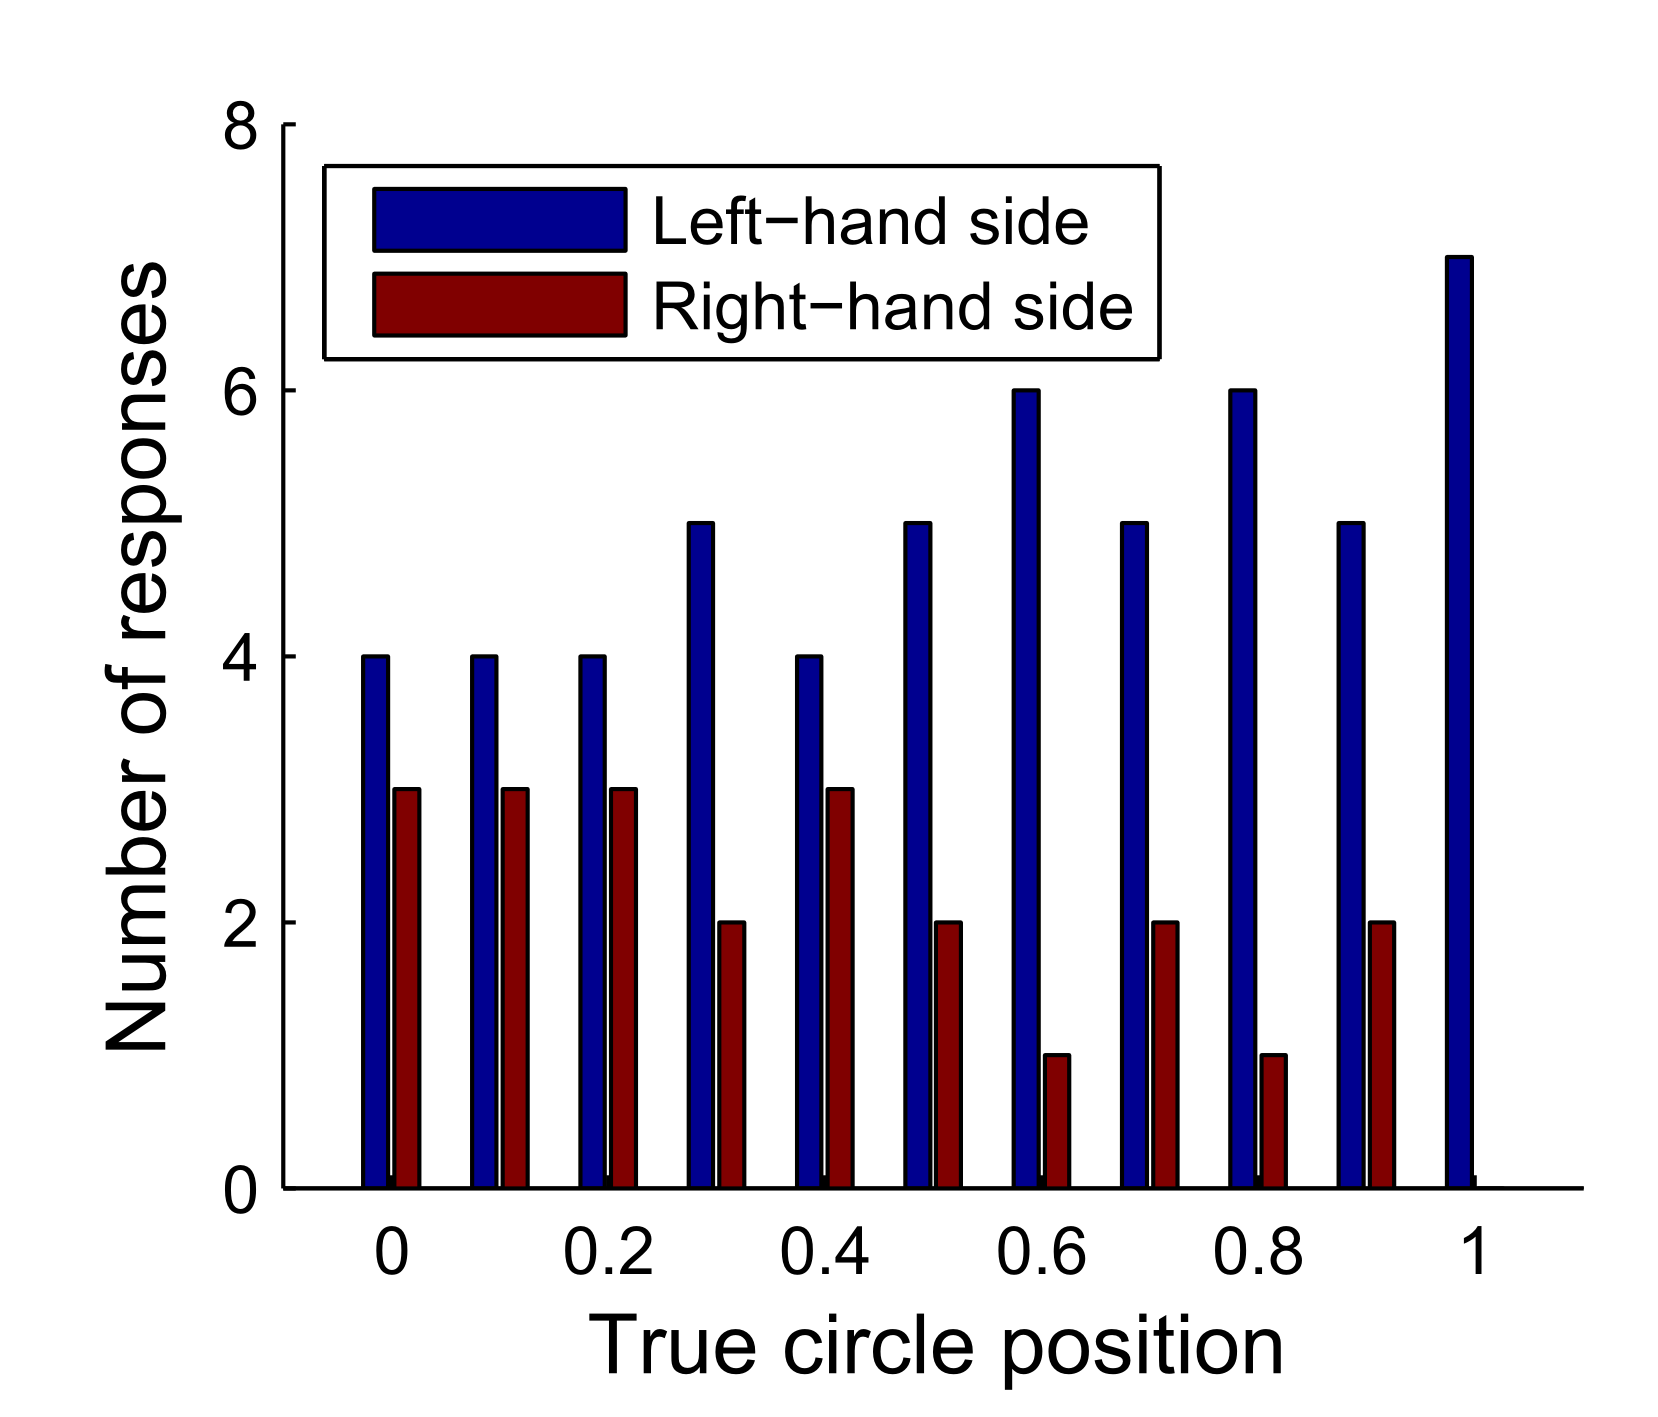
\includegraphics[scale=1]{bar_not_gold_responsesLR.png}
	\caption{}
	\label{Figure: bar_not_goldLR}	
	\end{subfigure}
	\label{Figure: not_gold_responsesLR}
	\caption{The number of left and right responses for the non-gold response workers. The total number of workers is 7.}
\end{figure}

The resulting dataset after gold filtering is shown in figure \ref{Figure:bar_gold_responsesLR}


\begin{figure}
	\centering
	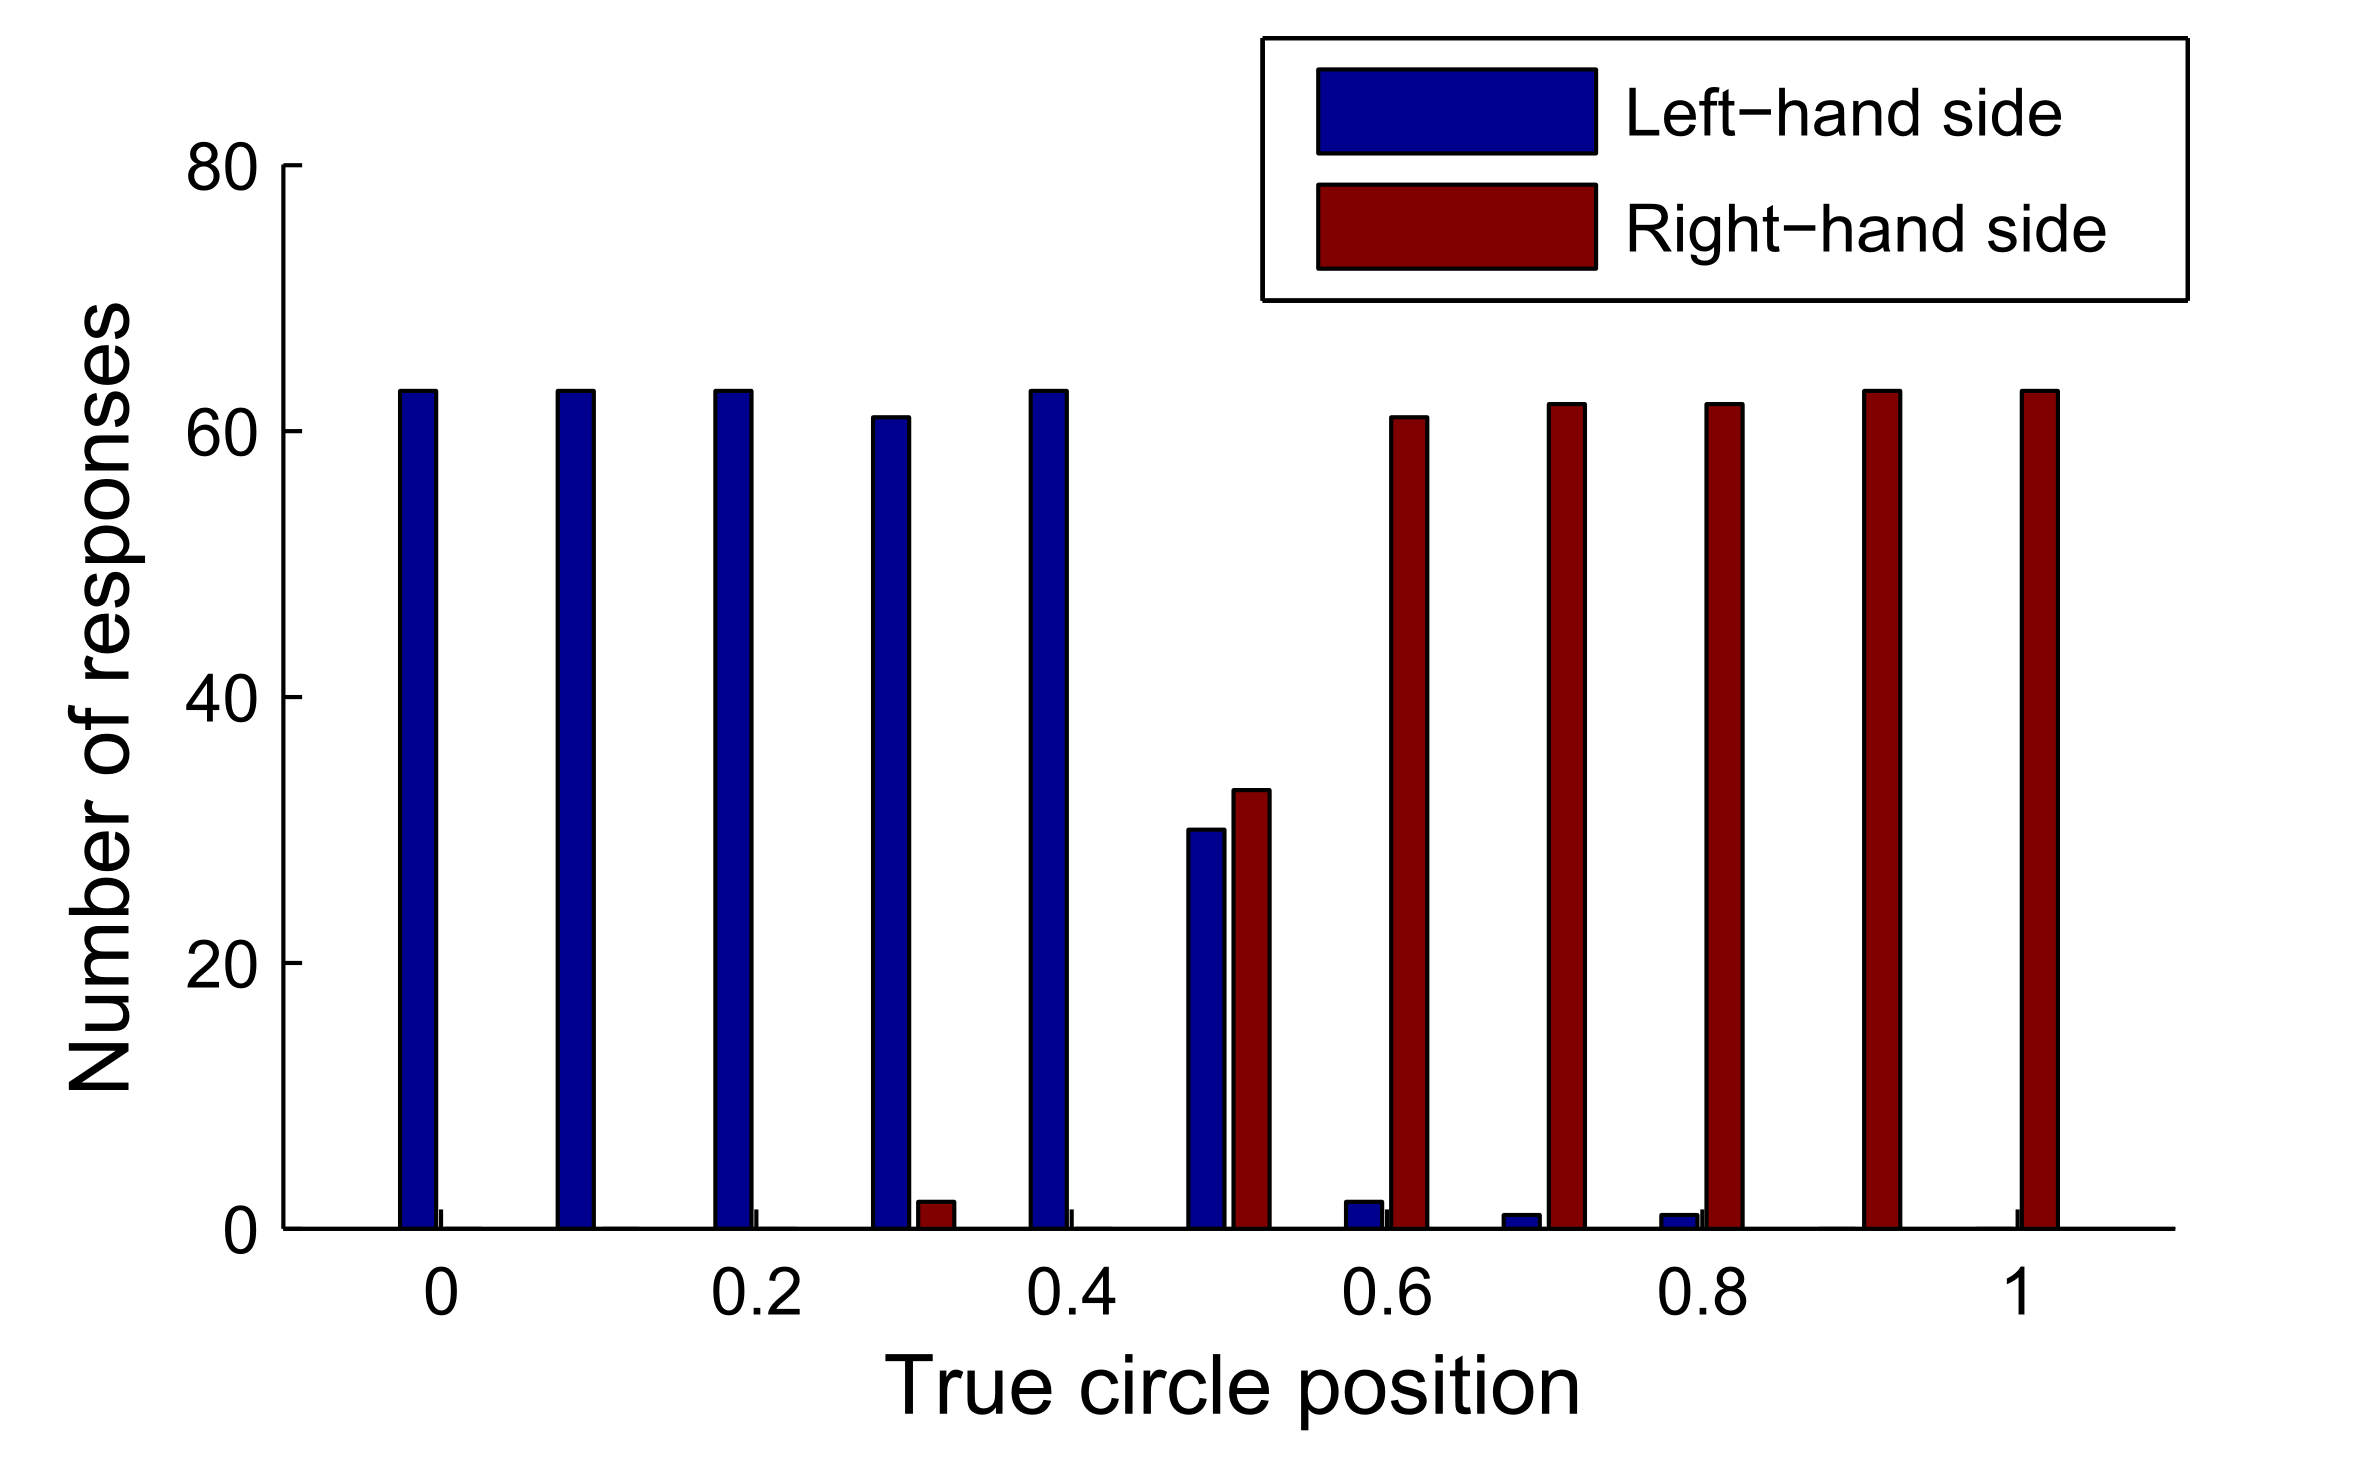
\includegraphics[scale=1]{bar_gold_responsesLR.png}
	\caption{The number of left and right responses at each circle position with gold filtering. The total number of workers is 63.}
	\label{Figure:bar_gold_responsesLR}
\end{figure}


\section{Softmax Function Fitting}

FIGURE shows the softmax function fit for the full dataset and gold standard dataset.



\section{Fusion Results}

\begin{figure}
	\centering
	\begin{subfigure}{7cm}
	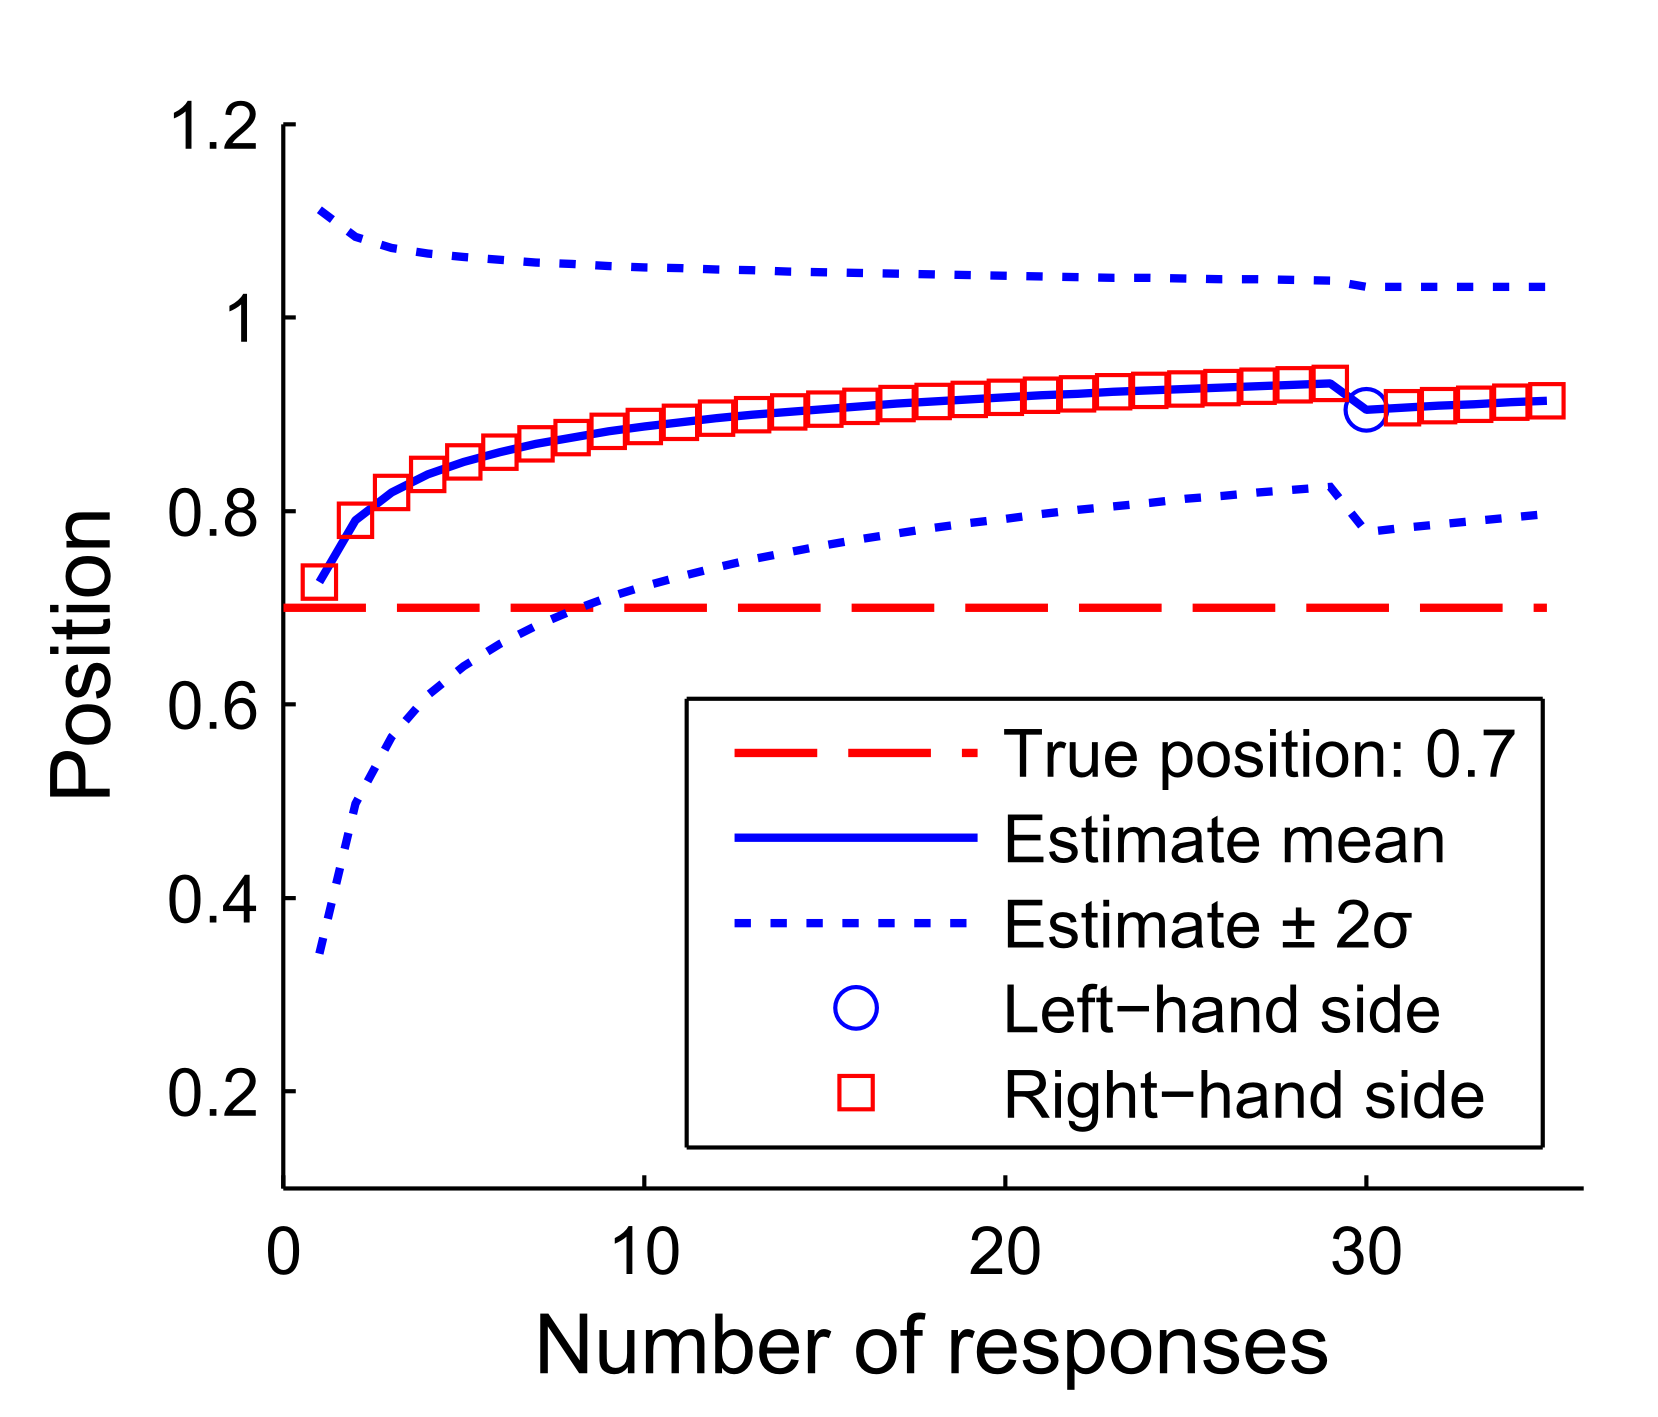
\includegraphics[scale=1]{line_fusion_responses_07_LR.png}
	\caption{}	
	\label{Figure: fusion_responses_07_varying_LR}
	\end{subfigure}
	\begin{subfigure}{7cm}
	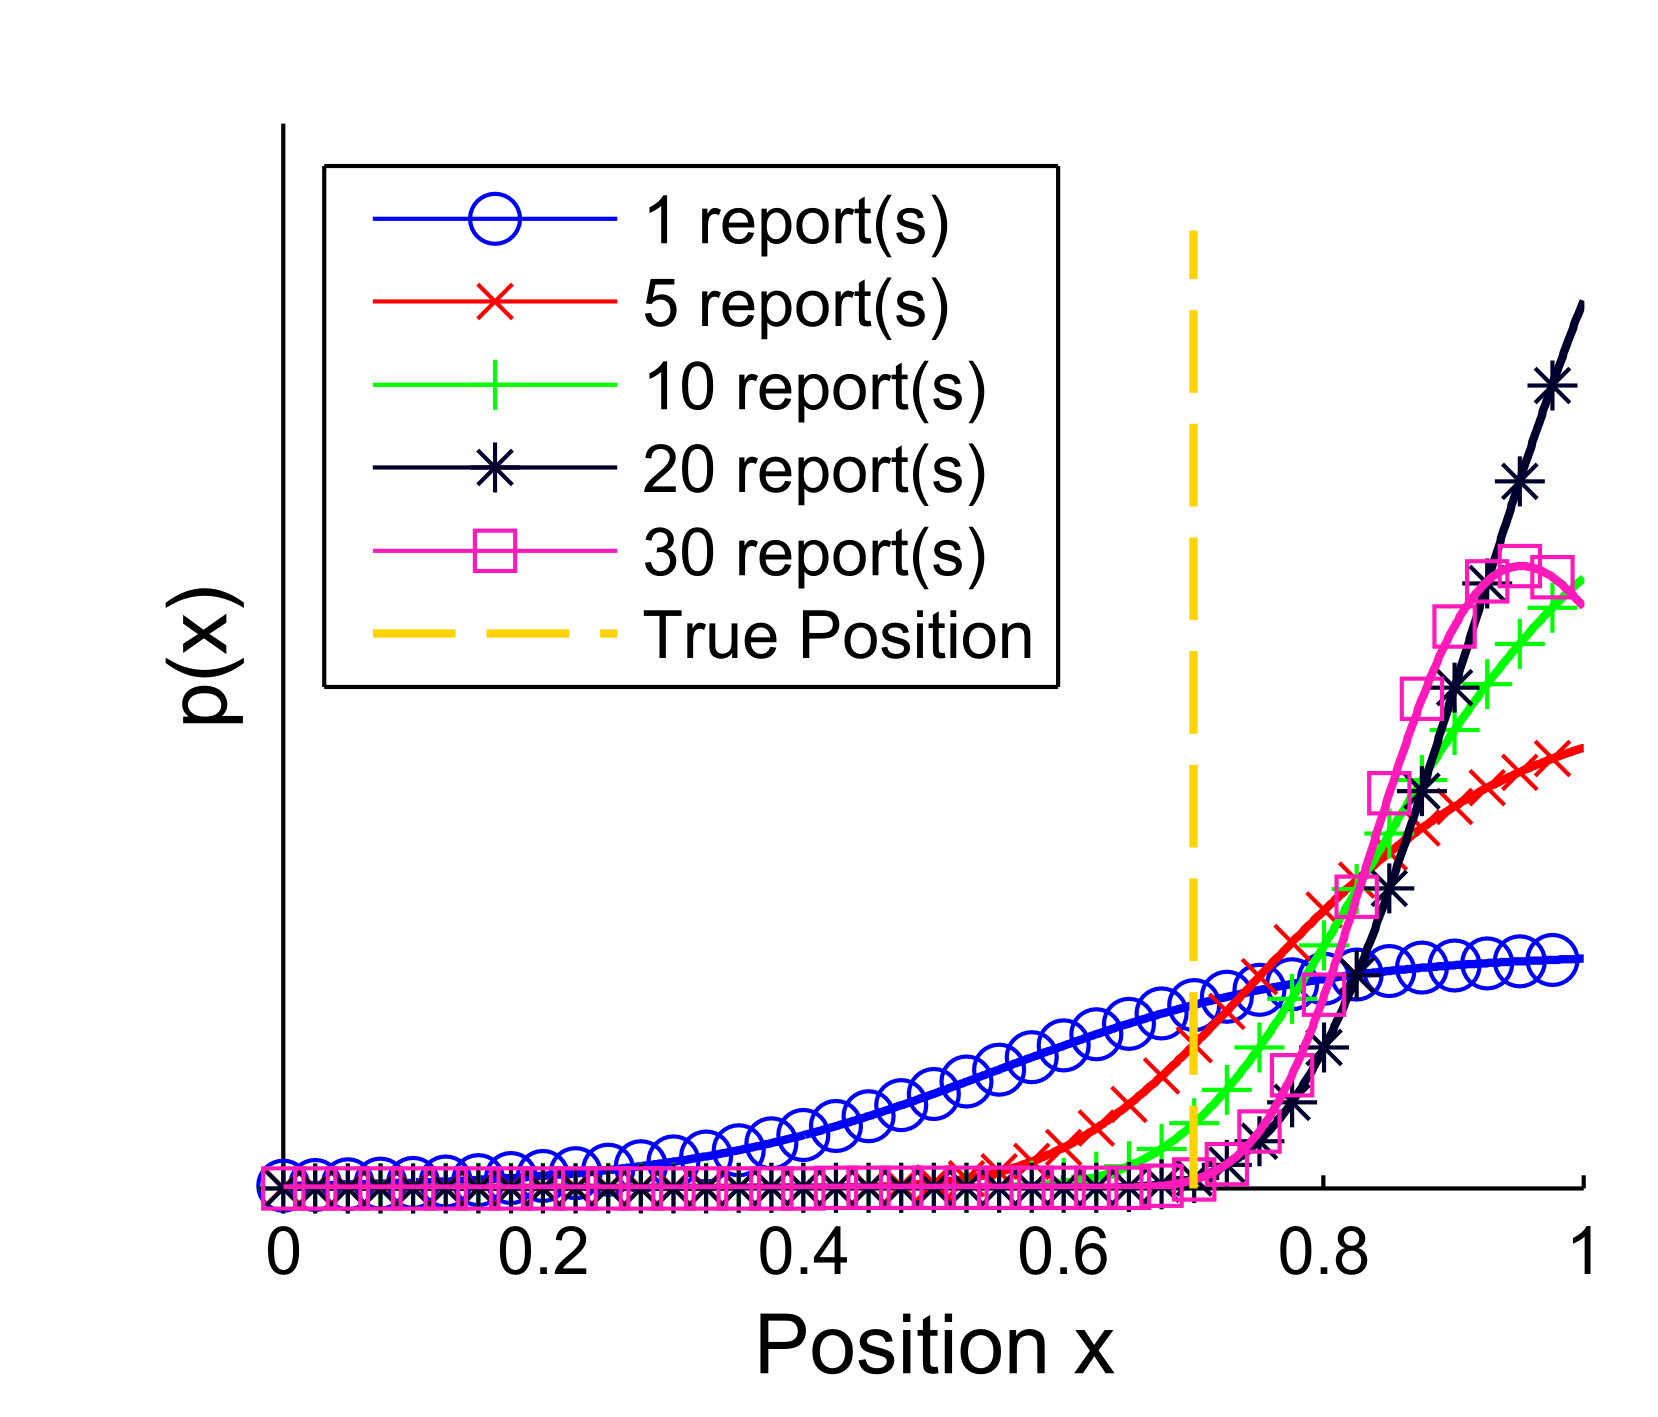
\includegraphics[scale=1]{line_fusion_07_distsLR.png}
	\caption{}
	\label{Figure: fusion_responses_07_dists_LR}	
	\end{subfigure}
	\label{Figure: fusion_responses_07_LR}
	\caption{Estimating the position of a circle as new reports are received \subref{Figure: fusion_responses_07_varying_LR}) The cahnge in posterior mean and standard deviation with responses \subref{Figure: fusion_responses_07_dists_LR}) Examples of the posterior distribution at different numbers of reports}
\end{figure}





\begin{figure}
	\centering
	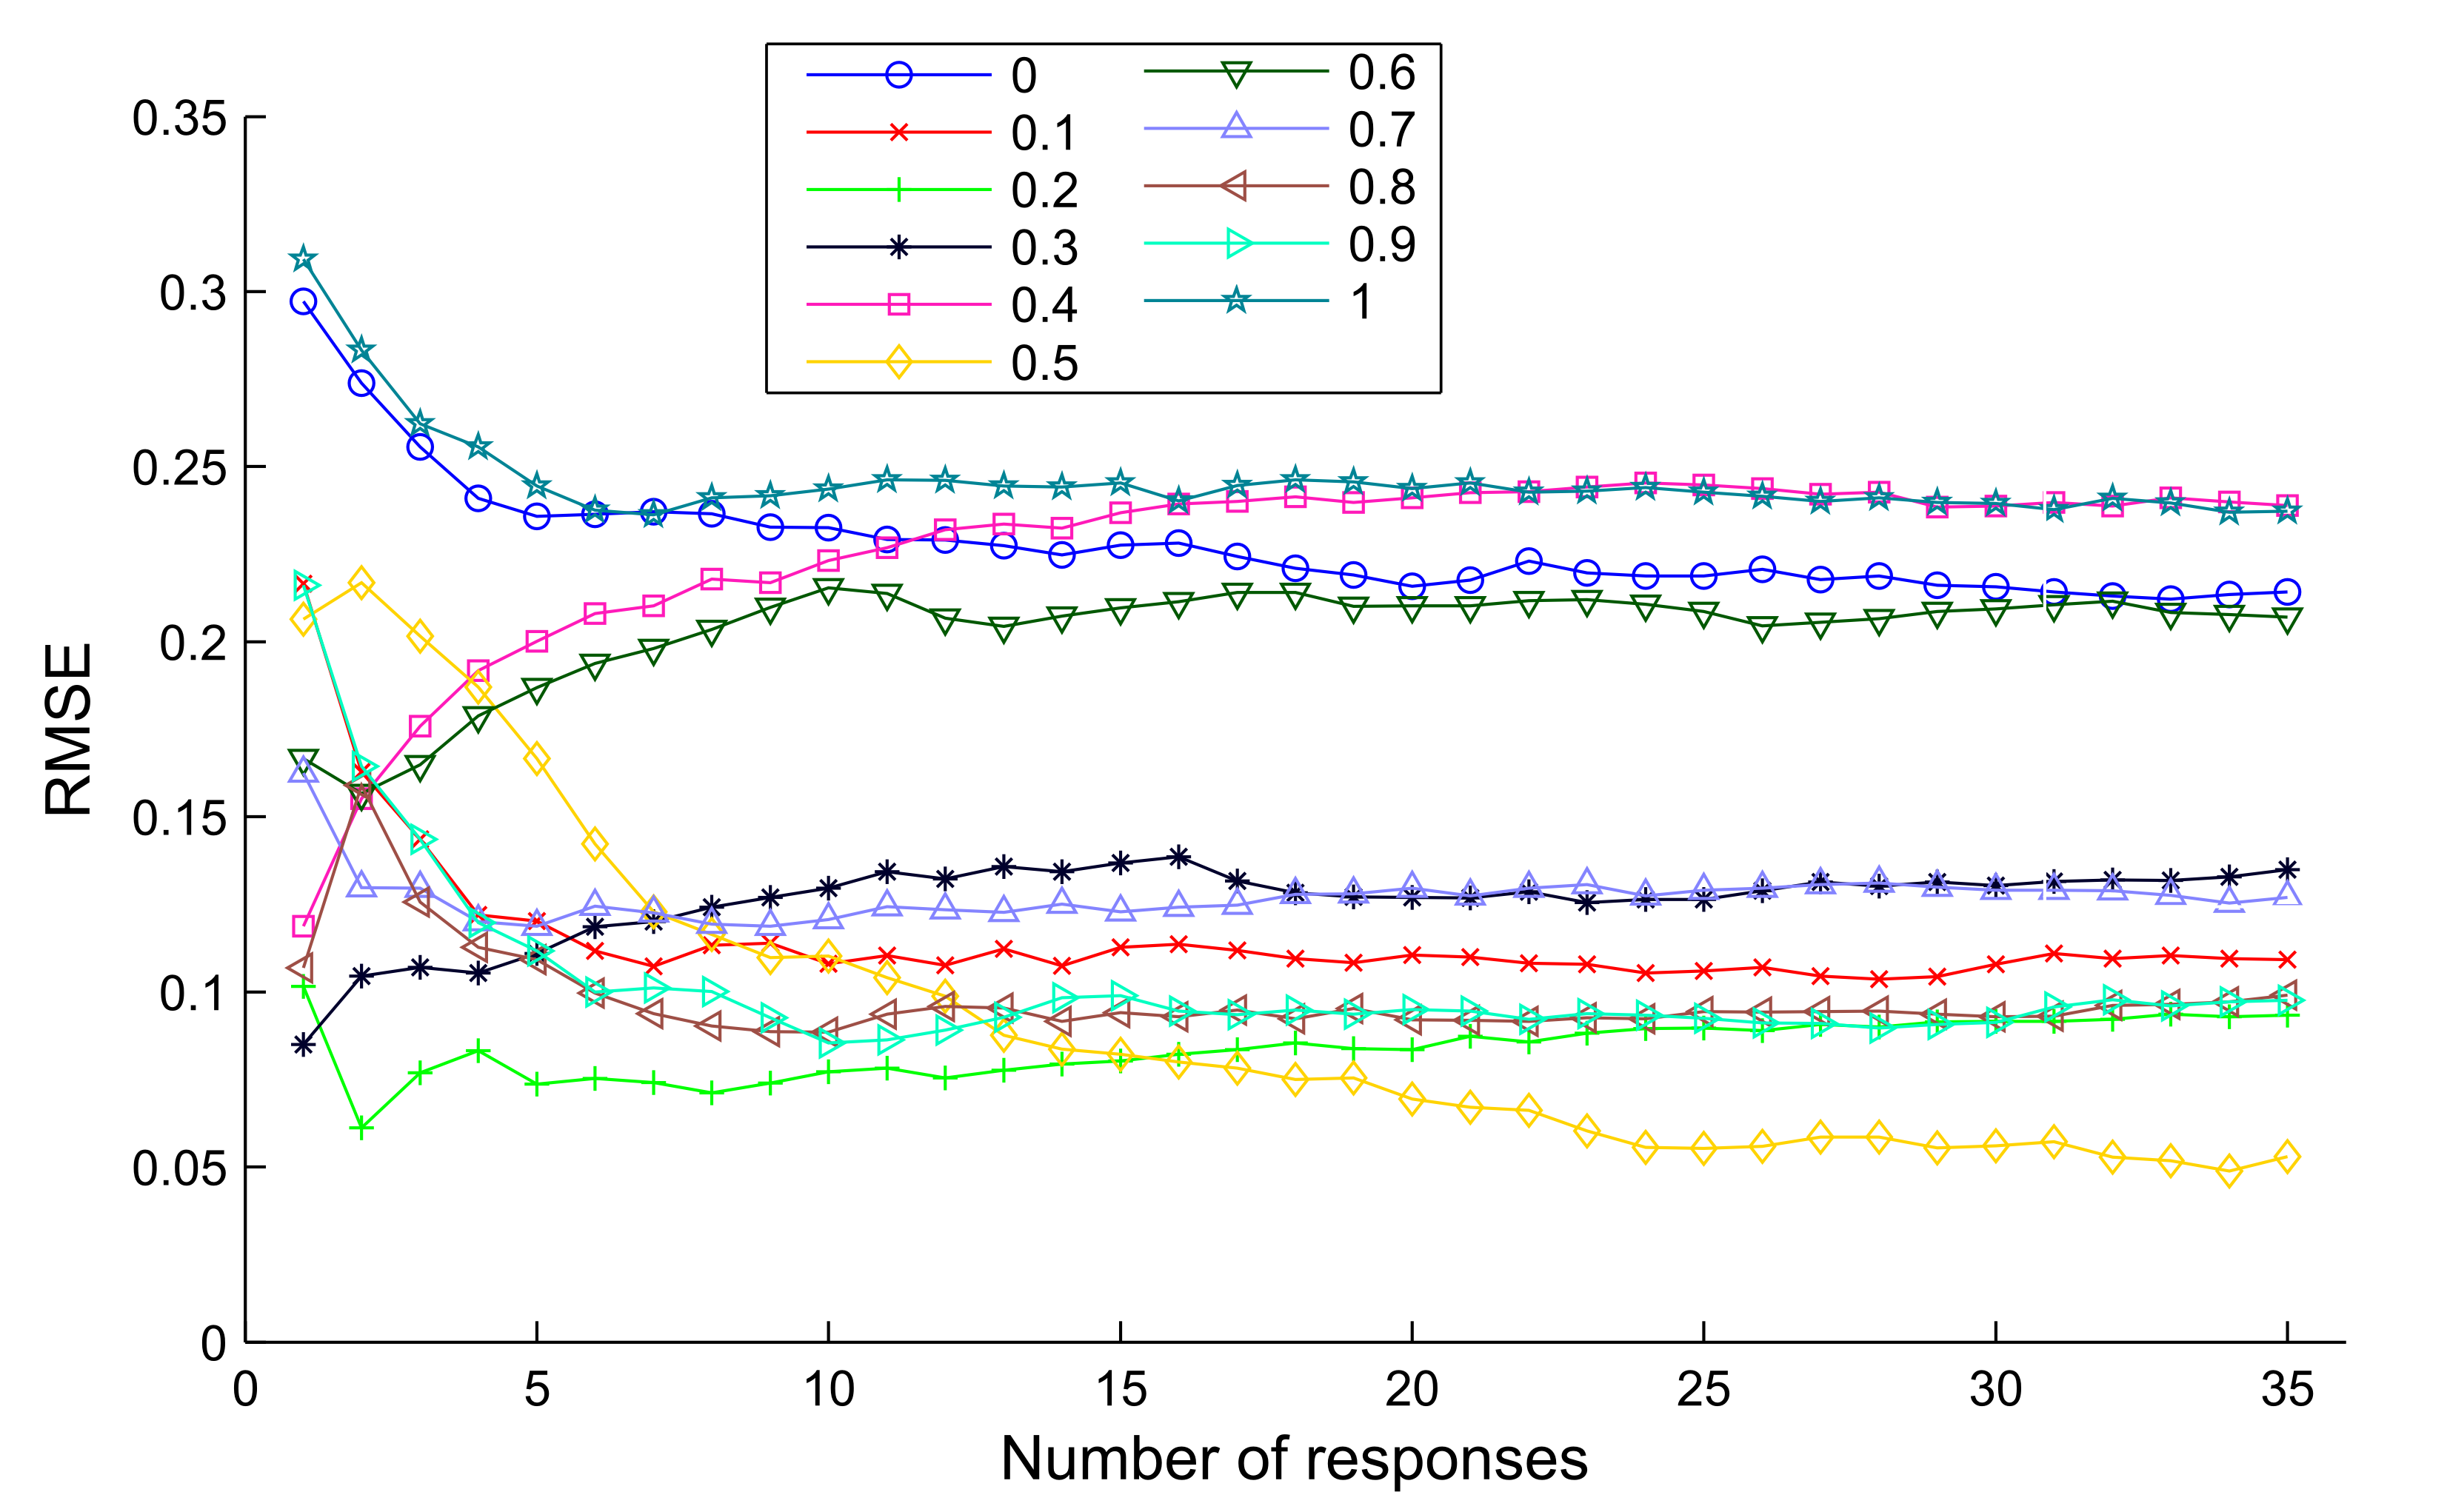
\includegraphics[scale=1]{line_fusion_RMSE_LR.png}
	\label{Figure: fusion_RMSE_LR }
	\caption{The RMSE at each circle position as the number of responses increases. The RMSE was generated over 50 simulation runs}
\end{figure}






\begin{figure}
	\centering
	\begin{subfigure}{7cm}
	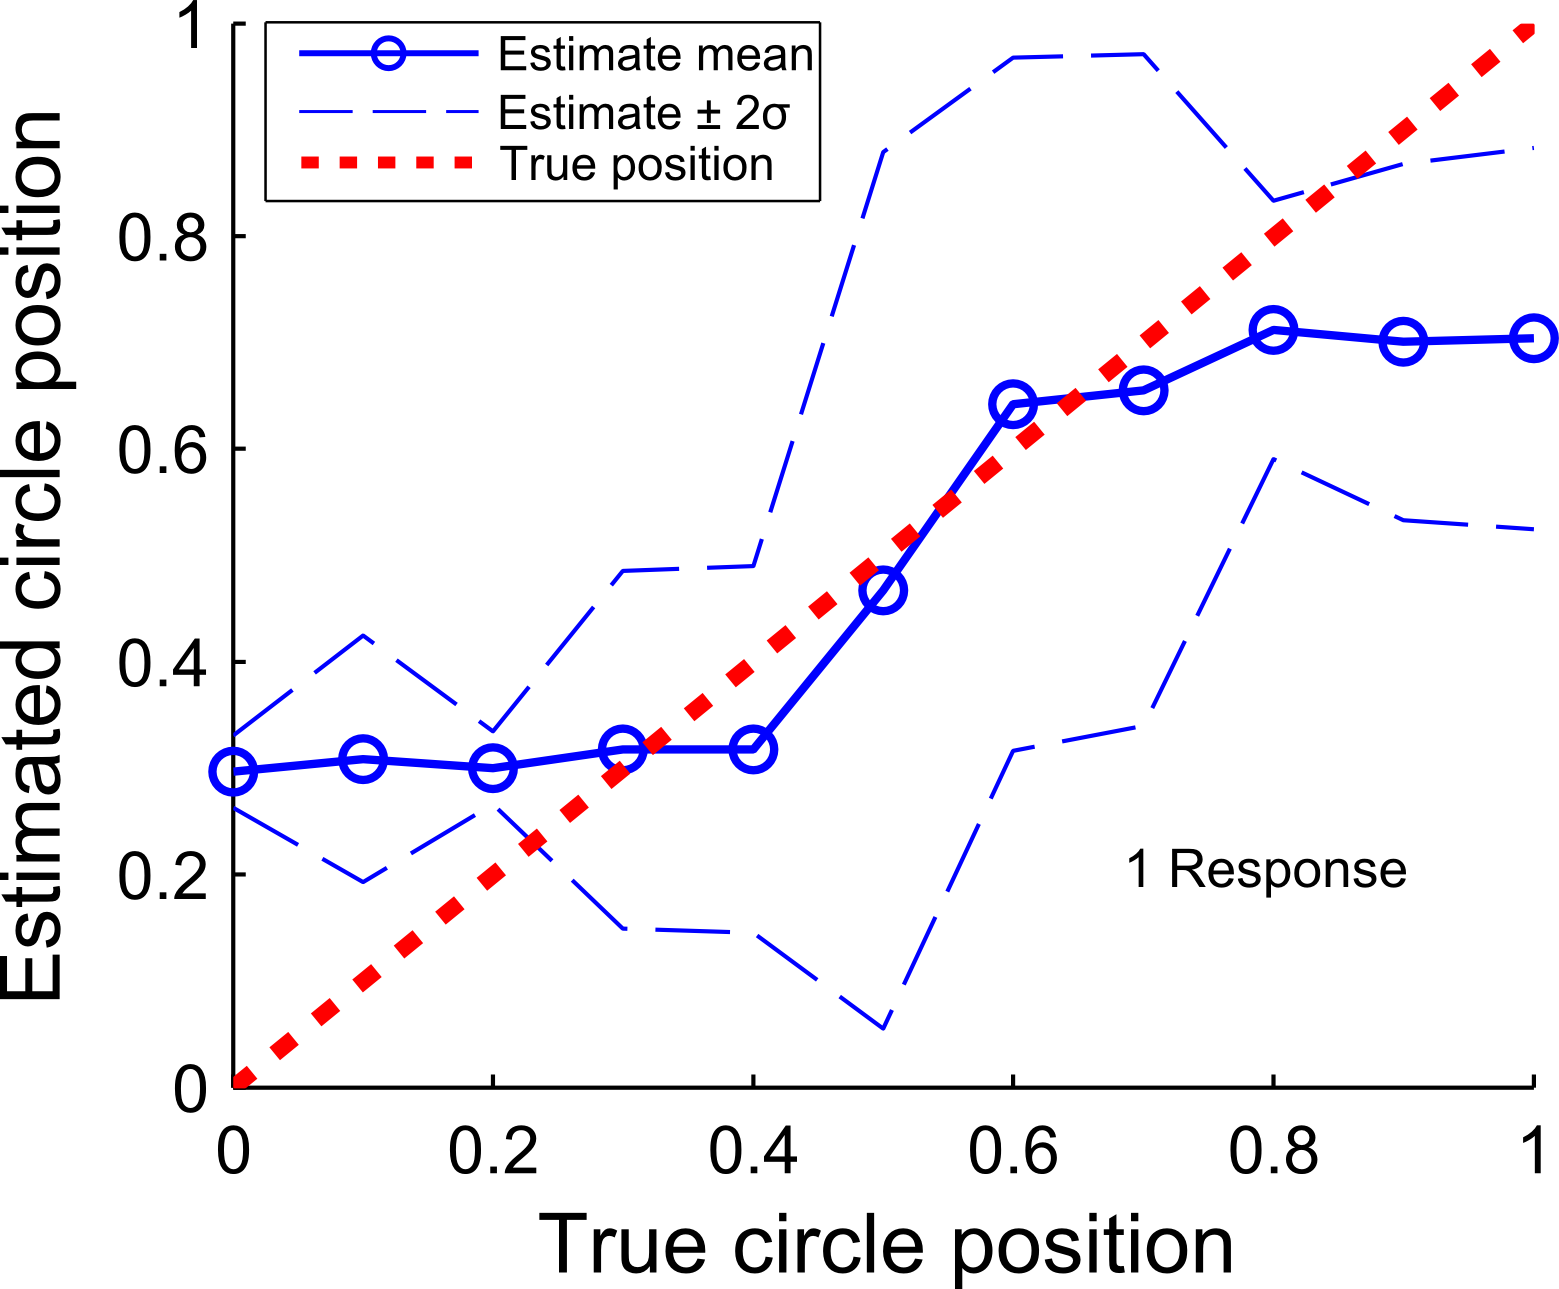
\includegraphics[scale=1]{line_fusion_mean_1rep_LR.png}
	\caption{}	
	\label{Figure: fusion_mean_1_LR}
	\end{subfigure}
	\begin{subfigure}{7cm}
	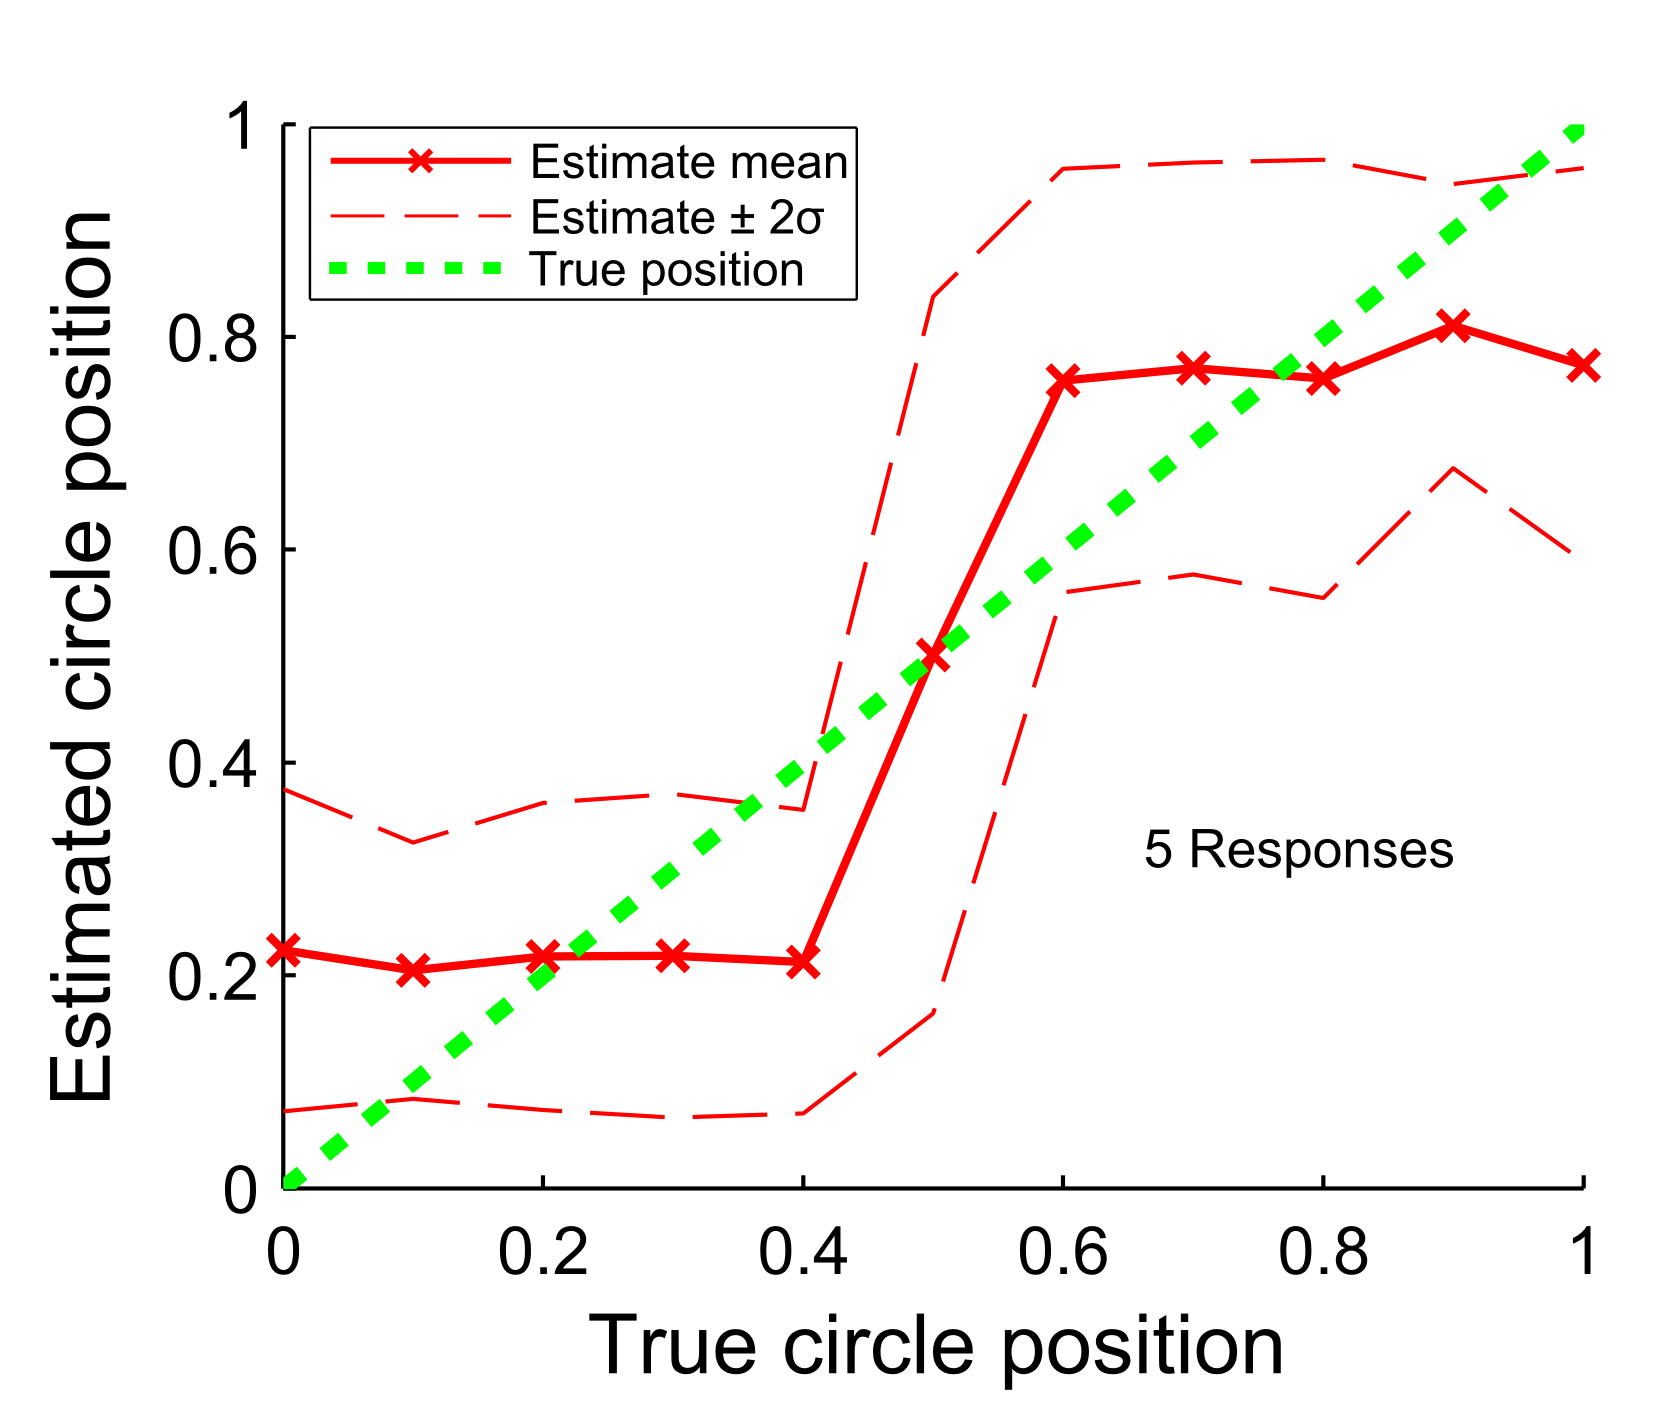
\includegraphics[scale=1]{line_fusion_5rep_LR.png}
	\caption{}
	\label{Figure: fusion_mean_5_LR}	
	\end{subfigure}\\
	\begin{subfigure}{7cm}
	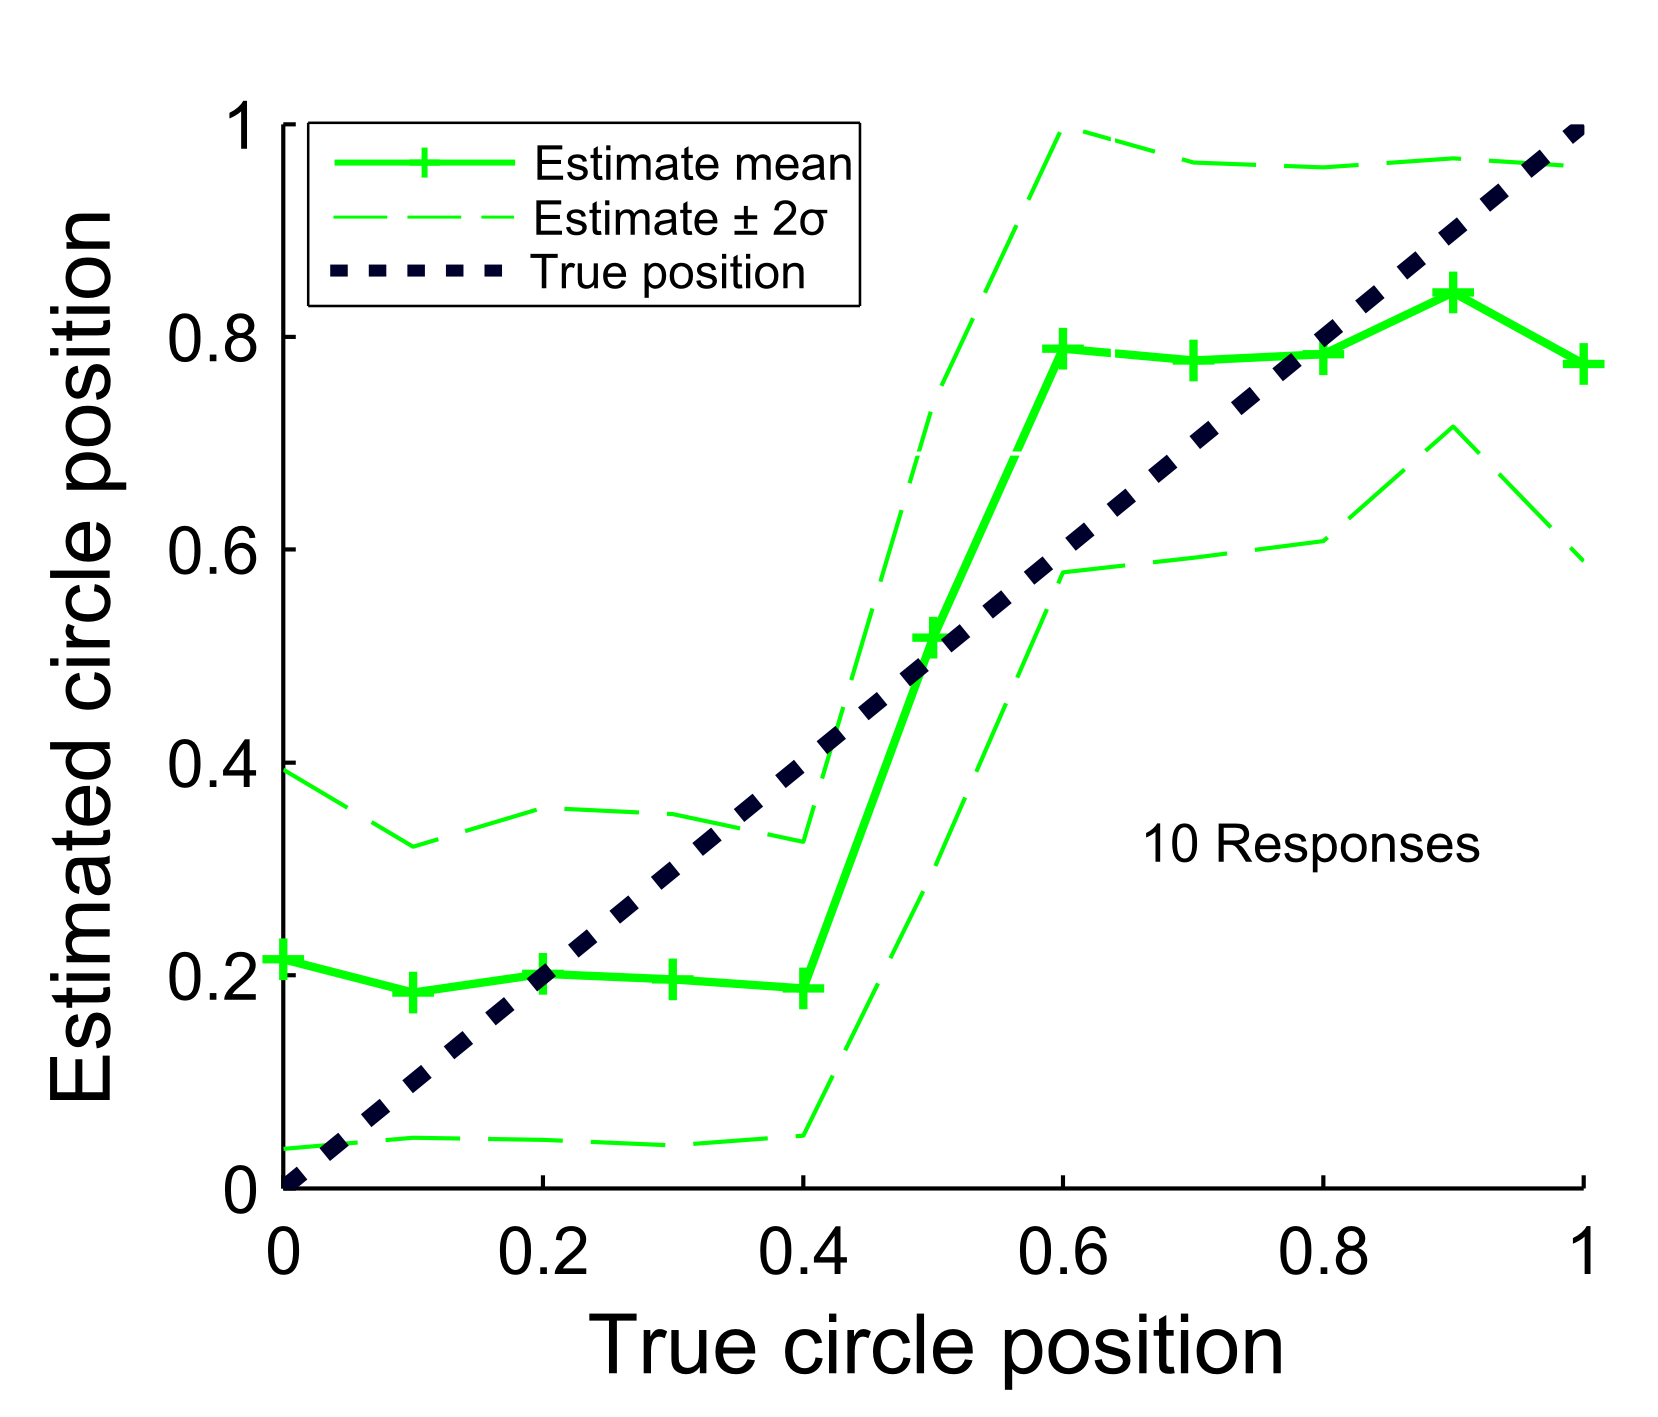
\includegraphics[scale=1]{line_fusion_10rep_LR.png}
	\caption{}	
	\label{Figure: fusion_mean_10_LR}
	\end{subfigure}
	\begin{subfigure}{7cm}
	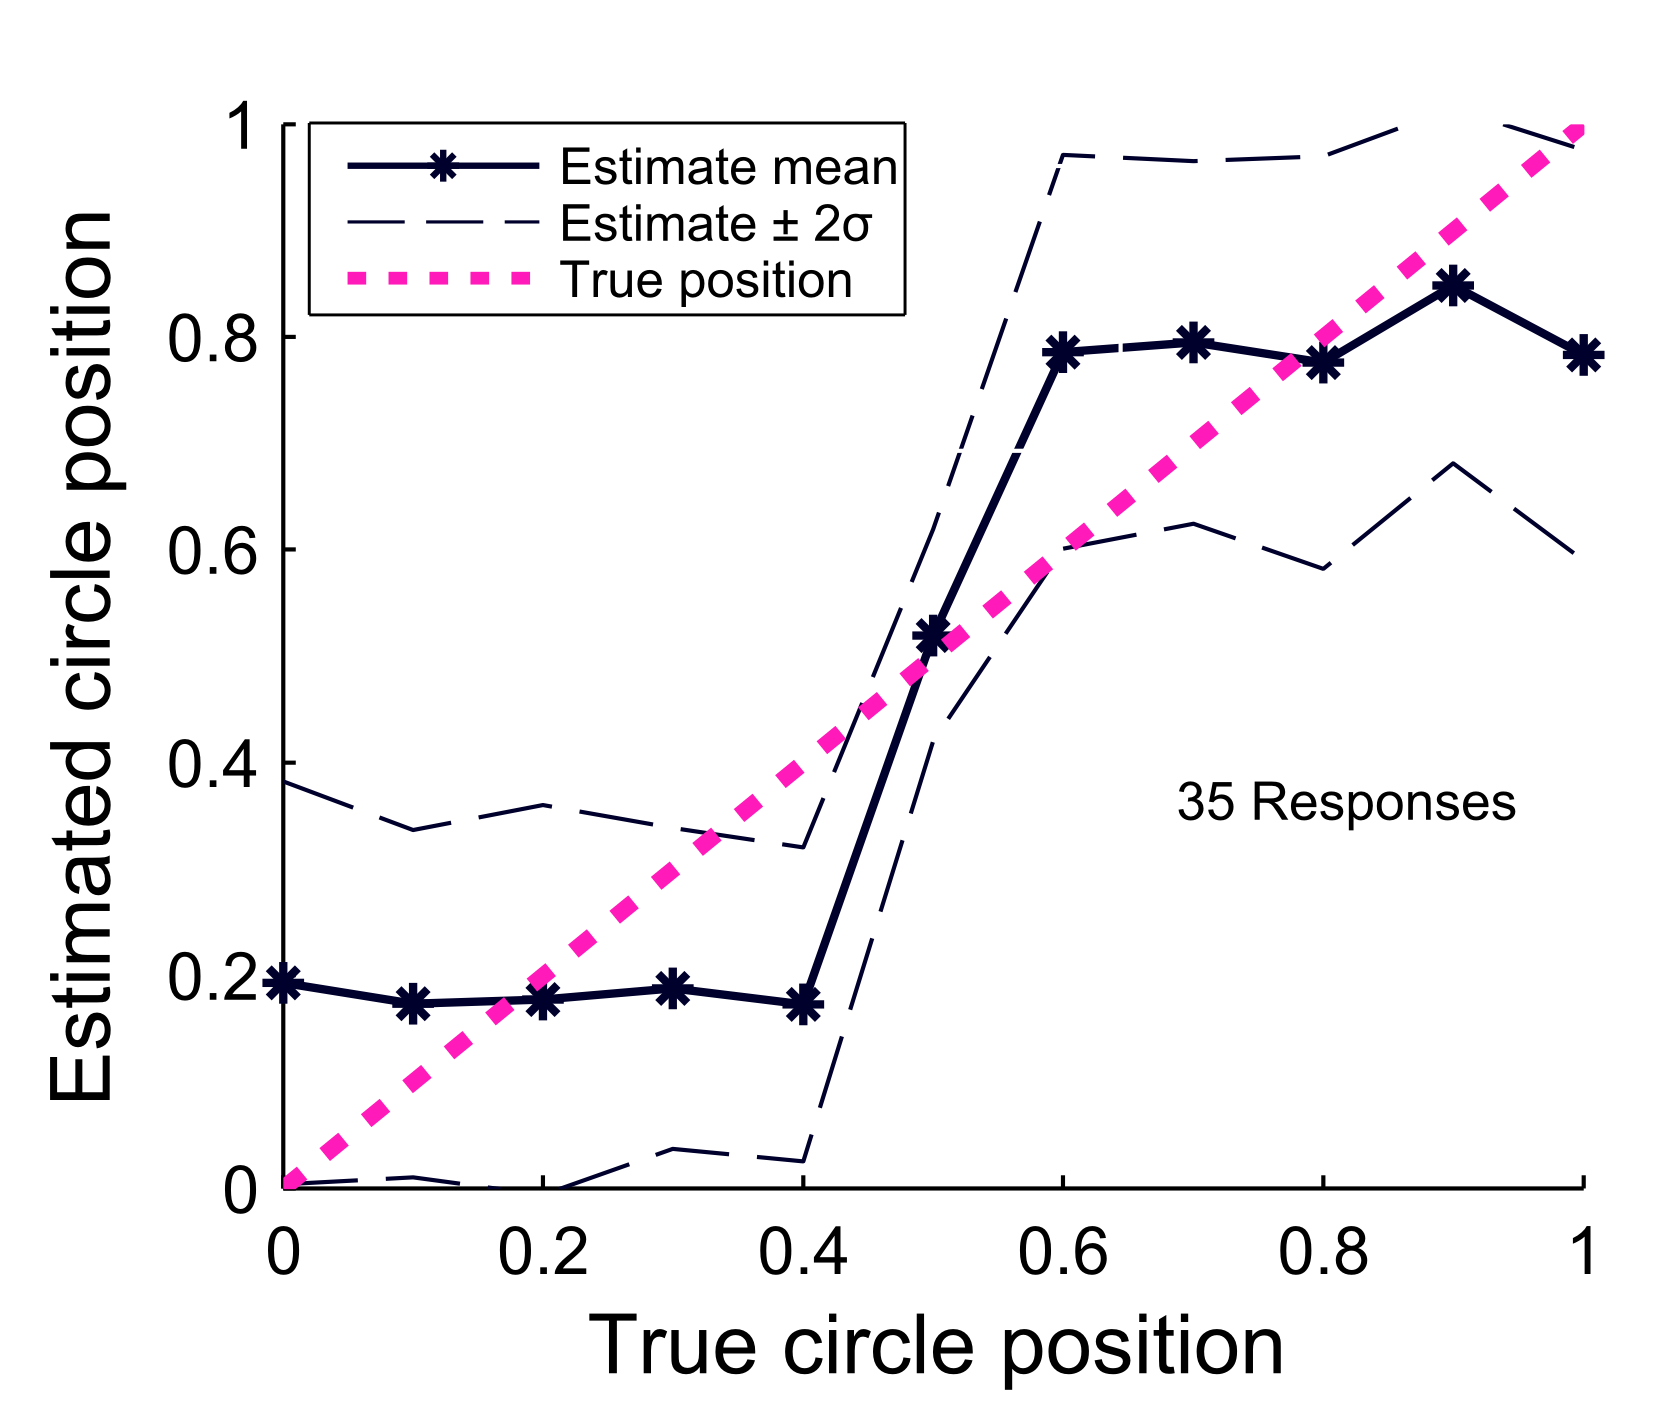
\includegraphics[scale=1]{line_fusion_35rep_LR.png}
	\caption{}	
	\label{Figure: fusion_mean_35_LR}
	\end{subfigure}
	\label{Figure: fusion_mean_LR}
	\caption{The mean performance of estimating the circle's position. The mean line is the expectation value of the posterior distribution taken from 50 simulations. The standard deviation is for the spread of expectation values over the simulations - not the spread in individual posteriors. The data was collected for varying numbers of responses with \subref{Figure: fusion_mean_1_LR}) 1 response \subref{Figure: fusion_mean_5_LR}) 5 responses \subref{Figure: fusion_mean_10_LR}) 10 responses \subref{Figure: fusion_mean_35_LR})35 responses}
\end{figure}